\documentclass[10pt]{article}
\usepackage[utf8]{inputenc}
\usepackage{mathptmx}
\usepackage{tabularx}
\usepackage{fancyvrb}
\usepackage{graphicx}
\usepackage{amsmath}
\usepackage{siunitx}
\usepackage{subcaption}
\usepackage[top=19mm, bottom=43mm, left=12.925mm, right=12.925mm, a4paper]{geometry}
\usepackage{hyperref}
\usepackage{xcolor}
\hypersetup{
    pdfpagelabels=true,
    plainpages=false,
    pdfauthor={Søren Bøgeskov Nørgaard, Henrik Aarup Vesterager, Lasse Thomsen},
    pdftitle={Satimo Python Library},
    pdfsubject={},
    bookmarksdepth=3,
    bookmarksnumbered=true,
    colorlinks,
    citecolor=black,
    filecolor=black,
    linkcolor=black,
    urlcolor=black,
    pdfstartview=FitH
}

\title{Satimo Python Library}
\author{Søren B.\ Nørgaard, Henrik A.\ Vesterager, Lasse Thomsen}
\begin{document}
\maketitle

\begin{abstract}
    This python 3 library makes it possible to extract data and calibrate measurements using trx-files exported directly from Satimo Passive Measurement.
\end{abstract}

\tableofcontents


\section{Files}
\begin{tabularx}{\linewidth}{lX}
    \texttt{cst.py} & Import CST files for manipulation/comparison. \\
    \texttt{l3d.py} & General 3D functionality (plotting, surface integration). \\
    \texttt{satimo.py} & Manipulation of data exported from Satimo Passive Measurement (SPM). 
\end{tabularx}

\section{Installation}
\begin{enumerate}
\item Make sure to install Python 3, numpy, scipy, and matplotlib.
\item Put the above files in a central directory (e.g.\ \texttt{C:/PathTo/Something}).
\item Add this path to the environment variable \texttt{PYTHONPATH} (\emph{Environment Variables} in Windows and \texttt{.bashrc} or \texttt{.profile} in Linux/OSX). E.g.\
    \begin{verbatim}
# ~/.profile
export PYTHONPATH=$PYTHONPATH:/home/soren/hdd/svn/project9-10/scripts/lib
    \end{verbatim}
\end{enumerate}


\section{Data Format}
The basic data format for a measurement is a $\theta \times \phi$-matrix for each frequency.
\begin{equation}
    M = \begin{bmatrix}
        m_{1,1} & m_{1,2} & \dots & m_{1,n} \\
        m_{2,1} & m_{2,2} & \dots & m_{2,n} \\
        \vdots & \vdots & & \vdots \\
        m_{m,1} & m_{m,2} & \dots & m_{m,n}
    \end{bmatrix}
\end{equation}
where $m$ is the number of $\theta$-elements (e.g.\ 15 for Satimo) and $n$ is the number of $\phi$-elements (e.g.\ 8 for Satimo). The angles matrix elements correspond to the following angles:
\begin{table}[htbp]
    \centering
    \begin{tabular}{|l|c|c|}
        \hline
        Elements & $\theta$ & $\phi$ \\
        \hline
        $m_{1,1}$ & \ang{0} & \ang{0} \\
        $m_{1,n}$ & \ang{0} & $\ang{360}$ \\
        $m_{m,1}$ & \ang{180}$^{\dagger}$ & \ang{0} \\
        \hline
    \end{tabular}
    \caption{Format of $\theta\times\phi$-matrix. $^{\dagger}$For Satimo measurements, this is $180-22.5=\ang{157.5}$ because of the blind spot in the bottom.}
    \label{tab:matrixformat}
\end{table}

\section{Modules}
\subsection{Satimo}
\subsubsection{col2mat(column, ntheta=SATIMO\_NUM\_ELEVATION, nphi=SATIMO\_NUM\_AZIMUTH)}
Convert a Satimo PM-exported column to a matrix with phi the 
x-axis and theta on the y-axis.

\begin{verbatim}
- column: Column from a Satimo PM export.
- ntheta: Number of rows in the output (theta in the input).
- nphi: Number of columns in the output (phi in the input).

Return:
Matrix with phi on the x-axis and theta on the y-axis.
\end{verbatim}

\subsubsection{efficiency(trxfile, calfiles, reffiles)}
Get the total efficiency of a trx file, exported from Satimo.

\begin{verbatim}
- trxfile: File, exported from Satimo PM, to compute the efficiency of.
- calfiles: List of calibration measurement files (trx files).
- reffiles: List of reference files relating to the calibration
        measurements.

Return:
[f,eff] -- the total efficiency, eff, for each frequency, f.
\end{verbatim}

\subsubsection{loadref(f)}
Load a reference file containing S11, Gain, and Efficiency of a
reference/calibration antenna.

\begin{verbatim}
- f: File name.

Return:
M[0]=frequency(Hz), M[1]=S11(.), M[2]=Gain(.), M[3]=Eff(.)
\end{verbatim}

\subsubsection{loadtrx(f)}
Load a trx measurement file from Satimo PM into memory. 

\begin{verbatim}
- f: TRX file to load.

Return:
[f, list_horiz, list_vert] where
        f = [f1, f2, f3, ...]
        list_horiz = [E_horiz_f1, E_horiz_f2, E_horiz_f3, ...]
        list_vert  = [E_vert_f1,  E_vert_f2,  E_vert_f3,  ...]
and each "E" is a complex matrix, (theta x phi), containing the received fields.
\end{verbatim}

\subsubsection{radiatedpower(h,v)}
Compute the radiated power for each frequency in the h and v list, using
radiatedpower\_single().

\begin{verbatim}
- h: List of complex (theta x phi) matrices -- one for each frequency.
        Horizontal polarization.
- v: List of complex (theta x phi) matrices -- one for each frequency.
        Vertical polarization.

Return:
A vector with the radiated power for each frequency/element of h and
        v.
\end{verbatim}

\subsubsection{radiatedpower\_single(Etot)}
Radiated power from a (theta x phi) total E-field matrix.

\begin{verbatim}
- Etot: Matrix (theta x phi) from Satimo PM to compute the radiate power
        of (surface integration).

Return:
Surface integral of Etot ~ radiated power.
\end{verbatim}

\subsubsection{totalpower\_table(calfiles, reffiles)}
Make a table of calibrated "total power" for each frequency.
Having (1) the total power and (2) the radiated power for a given antenna,
makes it possible to compute the total efficiency of the antenna.

\begin{verbatim}
- calfiles: List of calibration measurement files (trx files) (order:
        lowest to highest frequency).
- reffiles: List of reference files relating to the calibration
        measurements (order: lowest to highest frequency).

Return:
[f,Ptot] -- the total power for each frequency.
\end{verbatim}

\clearpage
\subsection{CST}
\subsubsection{col2mat(column, nx=360, ny=181)}
Convert a CST-exported column to a matrix with phi the 
x-axis and theta on the y-axis.

\begin{verbatim}
- column: Column from a Satimo export.
- nx: Number of columns in the output (phi in the input).
- ny: Number of rows in the output (theta in the input).

Return:
Matrix with phi on the x-axis and theta on the y-axis.
\end{verbatim}

\subsubsection{loadff(f)}
Load a CST exported file to two (theta x phi) matrices -- one for theta and
one for phi plarization.

\begin{verbatim}
- f: File to load.

Return:
[T,P] where T and P are each a (theta x phi) matrix.
\end{verbatim}

\clearpage
\subsection{L3D}
\subsubsection{ecc(Eth1, Eth2, Eph1, Eph2)}
Compute the envelope correlation coefficient between two farfields. The
farfields are split into theta and phi part. Each part is a matrix with
theta on one axis and phi on the other.

\begin{verbatim}
- Eth1: E-field, theta part, antenna 1
- Eth2: E-field, theta part, antenna 2
- Eph1: E-field, phi part, antenna 1
- Eph1: E-field, phi part, antenna 2

Return:
Envelope Correlation Coefficient (scalar)

Note:
https://mns.ifn.et.tu-dresden.de/Lists/nPublications/Attachments/612/Wang_Q_WSA_10.pdf
\end{verbatim}

\subsubsection{intsphere(r, theta, phi)}
Do a spherical integral of a theta-phi matrix.

\begin{verbatim}
- r: Matrix to integrate (x-axis=phi, y-axis=theta).
- phi: Phi axis values.
- theta: Theta axis values.

Return:
Scalar result of the integration.
\end{verbatim}

\subsubsection{plot3d(r, stride=1, th\_lim=(0, pi), ph\_lim=(0, 2*pi))}
Plot a matrix, (theta x phi), in 3d space.

\begin{verbatim}
- r: Matrix to plot.
- stride: Resolution of the output. 1=detailed+slow, 10=rough+fast.
- th_lim: Upper and lower theta limits.
- ph_lim: Upper and lower phi limits.
\end{verbatim}

\subsubsection{plotflat(r, th\_lim=(0,pi), ph\_lim=(0,2*pi), cmap="jet")}
Plot a farfield-matrix as a color-map. Remember that 0 degrees is the bottom
of the plot in spherical coordinates.

\begin{verbatim}
- r: Matrix to plot (theta x phi).
- th_lim: Minimum and maximum theta/y-axis value.
- ph_lim: Minimum and maximum phi/x-axis value.
- cmap: Color map to use.
\end{verbatim}



\clearpage
\section{Examples}
The file structure for these examples is as shown in Table~\ref{tab:example}. To run an example, e.g.\ \texttt{example1.py}, open the desired directory in a command prompt and type 
\begin{verbatim}
python example1.py
\end{verbatim}
\begin{table}[htbp]
    \centering
    \begin{tabular}{|l|l|}
        \hline
        File & Description \\
        \hline
        \texttt{example1.py}          & Efficiency example script. \\
        \texttt{example2.py}          & Plot 3D example script. \\
        \texttt{example3.py}          & CST farfield example script. \\
        \texttt{example4.py}          & Export efficiency as a text file example script. \\
        \texttt{example5.py}          & Plotting for IEEEtran example script.  \\
        \hline
        \texttt{cst\_farfield.txt}    & Farfield exported from CST. \\
        \texttt{antenna\_meas.trx}    & Antenna measurement (designed for 2400\,MHz). \\
        \hline
        \texttt{calib/calib2450.trx}  & Calibration measurement for 2450\,MHz dipole. \\
        \hline
        \texttt{calib/HomeRef500.ref} & Reference file for 500\,MHz dipole. \\
        \texttt{calib/HomeRef600.ref} & Reference file for 600\,MHz dipole. \\
        \texttt{calib/SD740-70.ref}   & Reference file for 740\,MHz dipole. \\
        \texttt{calib/SD850-02.ref}   & Reference file for 850\,MHz dipole. \\
        \texttt{calib/SD900-51.ref}   & Reference file for 900\,MHz dipole. \\
        \texttt{calib/SD1800-45.ref}  & Reference file for 1800\,MHz dipole. \\
        \texttt{calib/SD1900-49.ref}  & Reference file for 1900\,MHz dipole. \\
        \texttt{calib/SD2050-36.ref}  & Reference file for 2050\,MHz dipole. \\
        \texttt{calib/SD2450-43.ref}  & Reference file for 2450\,MHz dipole. \\
        \texttt{calib/SD2600-28.ref}  & Reference file for 2600\,MHz dipole. \\
        \hline
    \end{tabular}
    \caption{File structure for the example.}
    \label{tab:example}
\end{table}

\clearpage
\subsection{Extract Efficiency From Satimo}

The efficiency is extracted and plotted using the following script. The output is shown in Figure~\ref{fig:example1}.
\VerbatimInput{examples/example1.py}

\begin{figure}[htbp]
    \centering
    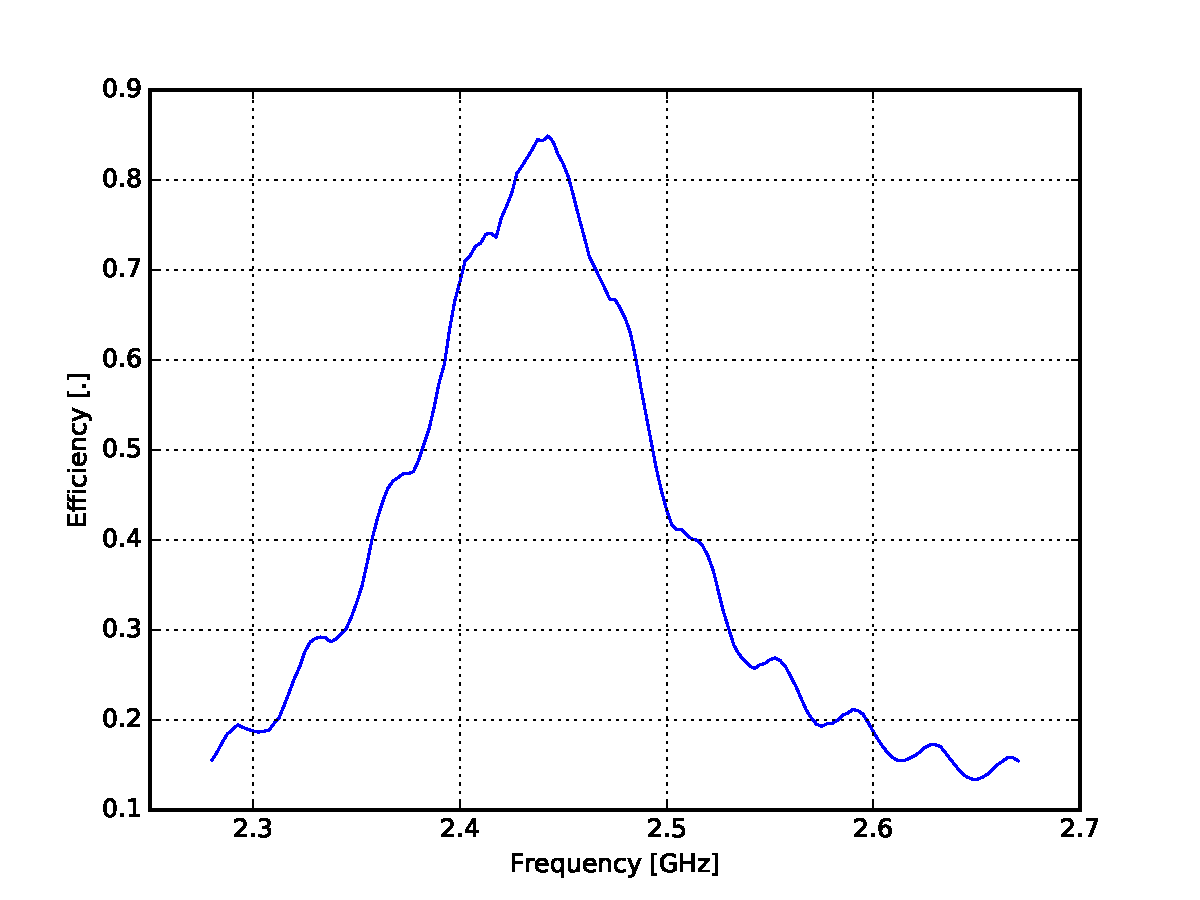
\includegraphics[scale=0.5]{examples/ex1_efficiency.pdf} 
    \caption{Efficiency plot from the example.}
    \label{fig:example1}
\end{figure}

\clearpage
\subsection{Plot 3D Farfield}

The (rough) farfield directly exported from Satimo's 15 probes can be plotted in 3D as shown below. The result is shown in Figure~\ref{fig:example2}. A similar plot -- a 2D color plot -- is also plotted.
\VerbatimInput{examples/example2.py}

\begin{figure}[htbp]
    \centering
    \begin{subfigure}{0.49\linewidth}
        \centering
        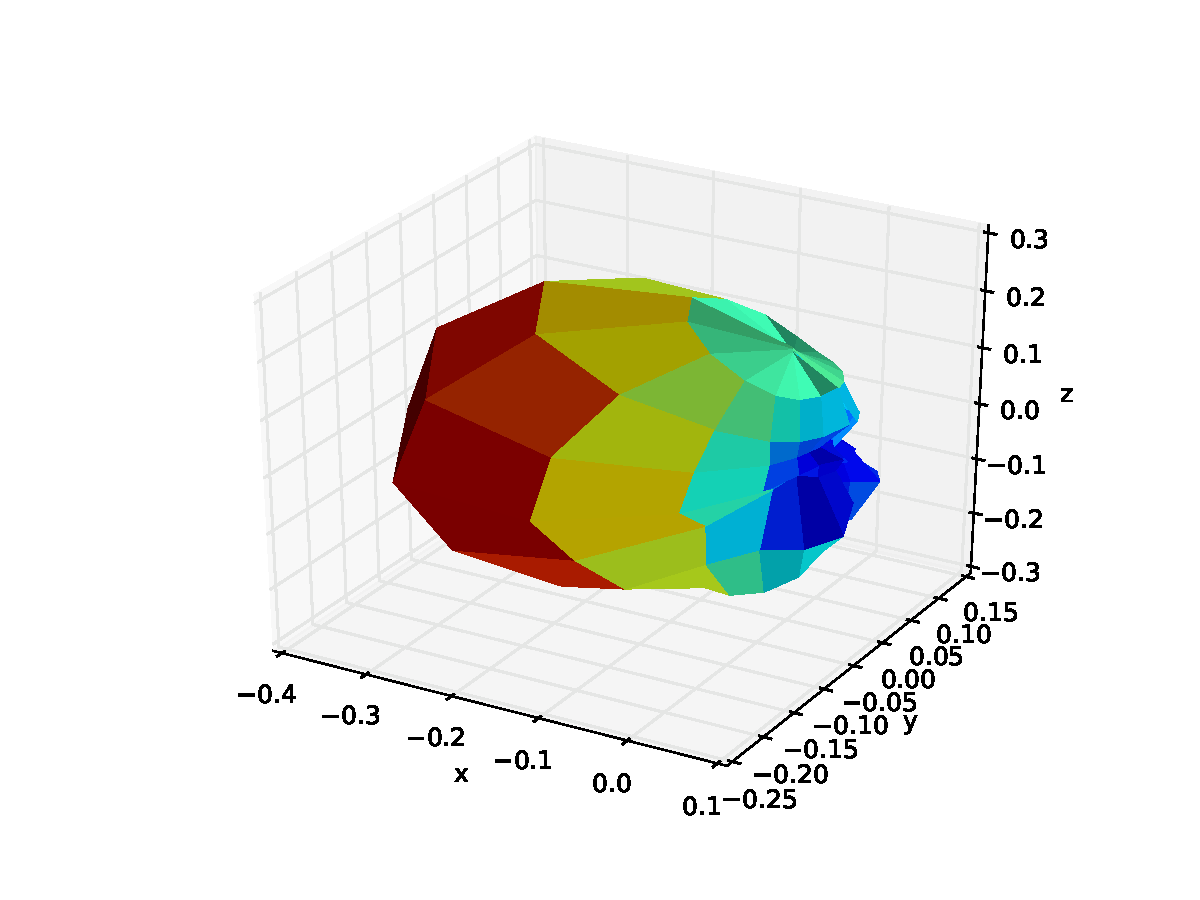
\includegraphics[scale=0.5]{examples/ex2_3dfarfield.pdf}
        \caption{3D.}
    \end{subfigure}
    \hfill
    \begin{subfigure}{0.49\linewidth}
        \centering
        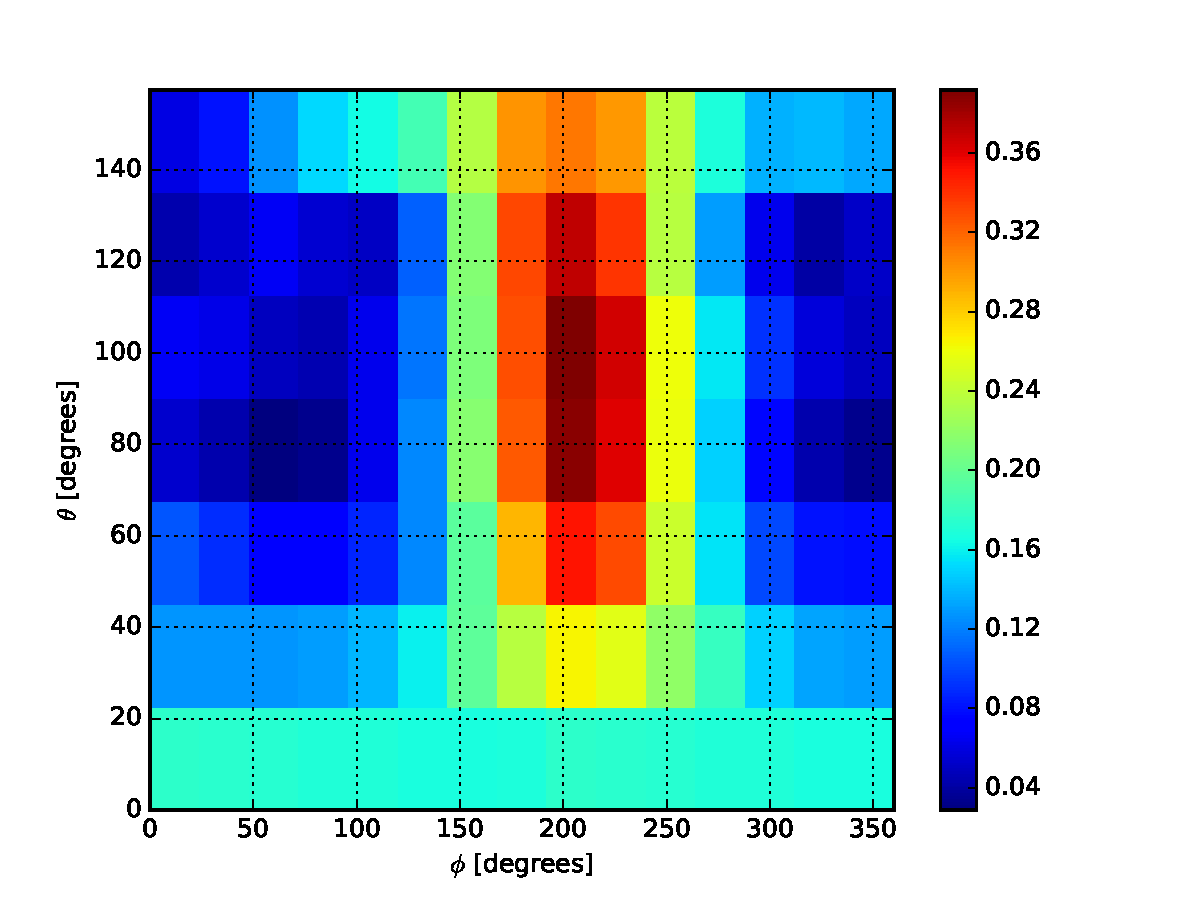
\includegraphics[scale=0.5]{examples/ex2_2dfarfield.pdf}
        \caption{2D.}
    \end{subfigure}
    \caption{Farfield plots.}
    \label{fig:example2}
\end{figure}

\clearpage
\subsection{Import a Farfield From CST}
The following example will import and plot a farfield from CST. The farfield should be exported under the Post Processing tab. The output is shown in Figure~\ref{fig:example3}.
\VerbatimInput{examples/example3.py}


\begin{figure}[htbp]
    \centering
    \begin{subfigure}{0.49\linewidth}
        \centering
        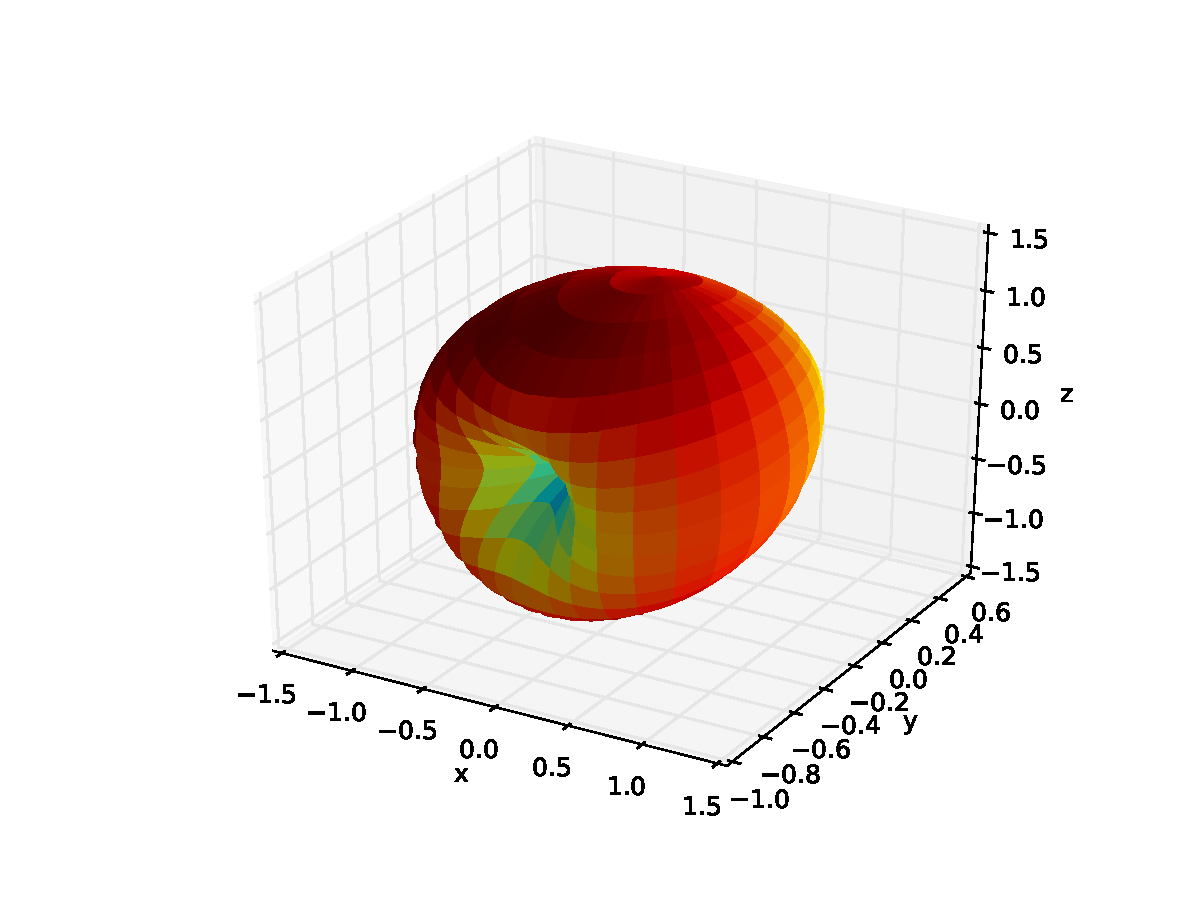
\includegraphics[scale=0.5]{examples/ex3_3dfarfield.pdf}
        \caption{3D.}
    \end{subfigure}
    \hfill
    \begin{subfigure}{0.49\linewidth}
        \centering
        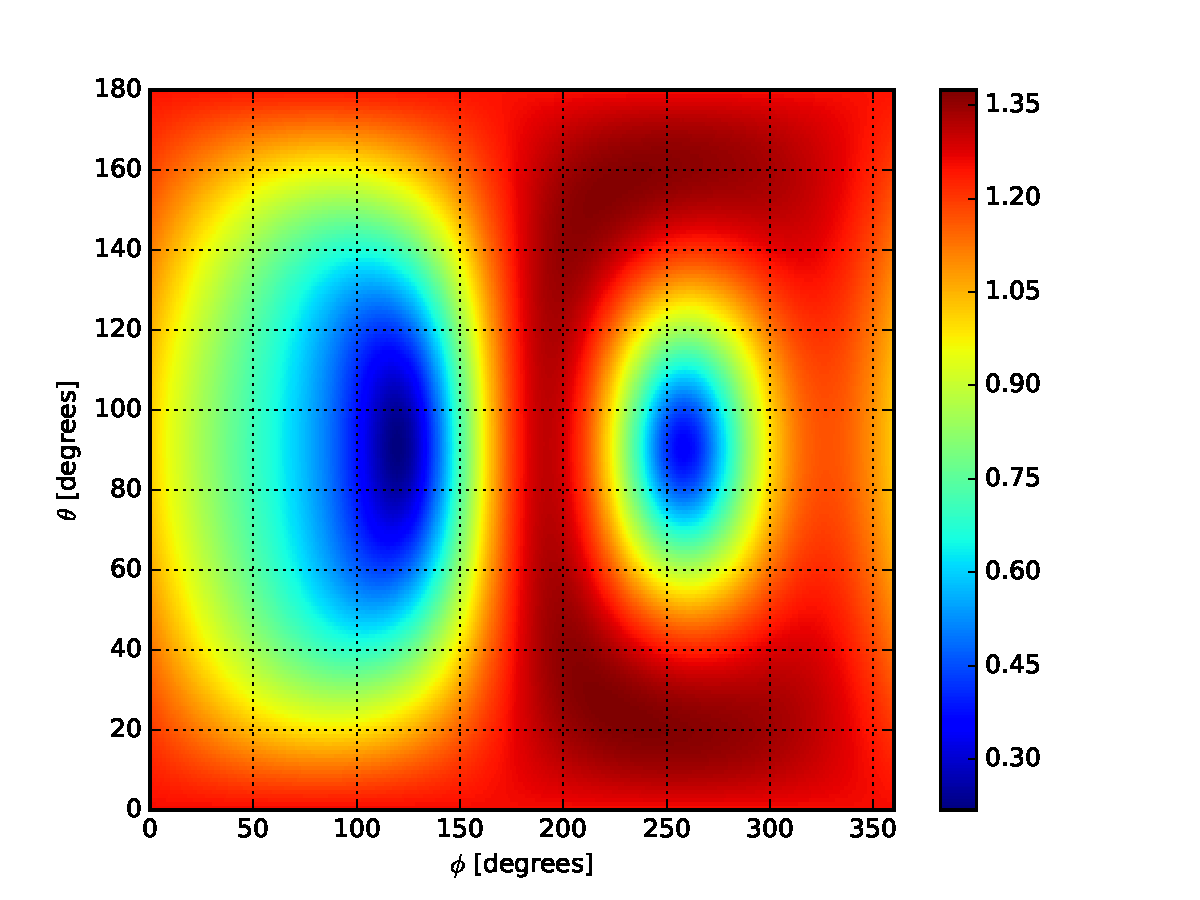
\includegraphics[scale=0.5]{examples/ex3_2dfarfield.pdf}
        \caption{2D.}
    \end{subfigure}
    \caption{Farfield plots.}
    \label{fig:example3}
\end{figure}

\clearpage
\subsection{Export Efficiency for Further Analysis}

Using python and numpy, analysis and comparison can be done just as easily as in MATLAB. However, if one is more familiar with MATLAB or need the data for other software, it is advantageous to export the data. Here is a simple example of exporting the efficiency as a data file.
\VerbatimInput{examples/example4.py}

The output is a tab-separated file (\texttt{ex4\_efficiency.txt}) which can easily be imported into MATLAB or similar software.


\clearpage
\subsection{Plots for IEEEtran Articles}
It is often desirable to export graphs in a format that is compliant with the text used articles. In the standard IEEEtran format, a \emph{Times} font is used. For figures, the default font size is 8\,pt. The column width is \SI{3.5}{inches}. In the example, the figure size is set to $\SI{3.5}{inches}\times \SI{3}{inches}$.

Note that math symbols can easily be used in figure text (e.g.\ labels) in the same way as symbols are written in \LaTeX, e.g.\ ``\verb|$\theta$ in degrees|'' becomes ``$\theta$ in degrees''.

The result is shown in Figure~\ref{fig:example5}.

\VerbatimInput{examples/example5.py}

\begin{figure}[htbp]
    \centering
    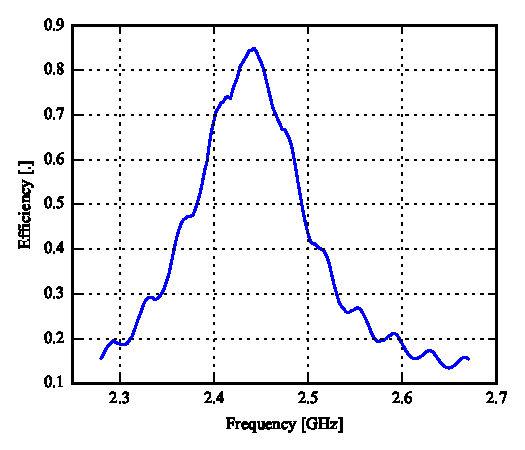
\includegraphics{examples/ex5_efficiency.pdf}
    \caption{Efficiency plot in IEEEtran format.}
    \label{fig:example5}
\end{figure}

\end{document}
